\section{Método de Householder para Matrizes Simétricas}

Considere o operador de \textit{Householder} dado por:

\begin{equation}
\label{cap5:sec3:eq1}
[P] = [I] - 2 \, \{e\} \, \{e\}^T
\end{equation}

onde $ \{e\} $ é um vetor unitário, isto é, $ \, \{e\} \, \cdotp \{e\} = 1 $.

Considere o produto $ [P] [P]^T = [M] $. Assim,

\begin{equation}
\label{cap5:sec3:eq2}
 M_{ij} = P_{ik} \, P_{kj}^T = P_{ik} \, P_{jk} = (I_{ik} - 2 \, e_i \, e_k) \, (I_{jk} - 2 \, e_j \, e_k)
\end{equation}

\textbf{OBS:} Assumimos que índices repetidos no monômio implicam $ \displaystyle \sum_1^n $.

\equacao {
\begin{array}{ll}
 M_{ij} & = I_{ik} \, I_{jk} - 2 \, I_{ik} \, e_j \, e_k - 2 \, e_i \, e_k \, I_{jk} + 4 \, e_i \, e_j \underbrace{e_k \, e_k}_{1} \\
 & = \mbox{ $ I_{ij} - 2 \, e_j \, e_i - 2 \, e_i \, e_j + 4 \, e_i \, e_j $ } \\
 & = \delta_{ij} - 4 \, e_i \, e_j + 4 \, e_i \, e_j = I_{ij} \\
\end{array}
}

\begin{equation}
\label{cap5:sec3:eq3}
 [M] = [I] \Rightarrow [P] \, [P]^T = [I]
\end{equation}

Logo $ [P]^T = [P]^{-1} \Rightarrow [P] $ \underline{é ortogonal (ortonormal)}.

$ [P] $ é simétrica?

\begin{equation}
 P_{ij} = \delta_{ij} - 2 \, e_i \, e_j = \delta_{ji} - 2 \, e_j \, e_i = P_{ji}
\end{equation}

Assim, $ [P] = [P]^T \Rightarrow [P] $ \underline{é simétrica}.

Considere a transformação de um vetor $ \{a\} $ pelo operador de \textit{Householder}:

\begin{equation}
\label{cap5:sec3:eq5}
 [P] \, \{a\} = \{b\}
\end{equation}

Vamos criar o vetor $ \{e\} $ em \ref{cap5:sec3:eq1} a partir do vetor $ \{a\} $ como se segue:

\begin{enumerar}

\item Defina $ s $ como o comprimento de $ \{a\} $. Assim,

\begin{equation}
 s = \sqrt{\{a\} \cdotp \{a\}} = \sqrt{\{a\}^T \, \{a\}}
\end{equation}

\item Defina um vetor $ \{c\} $ tal que

\begin{equation}
 \{c\} = \{a_1 + s \mbox{(sinal de $ a_1 $)} , a_2, a_3, \ldots, a_n\}
\end{equation}

\item Defina $ \{e\} $ como o vetor unitário na direção de $ \{c\} $:

\begin{equation}
 \{e\} = \frac{\{c\}}{\sqrt{\{c\}^T \, \{c\}}} = \frac{\{c\}}{|\{c\}|}
\end{equation}

\end{enumerar}

Verifiquemos o que ocorre com a transformação \ref{cap5:sec3:eq5}:

\begin{equation}
\label{cap5:sec3:eq9}
 [P] \, \{a\} = \left[ I - 2 \, \frac{c \, c^T}{c^T \, c} \right] \, \{a\} = \{a\} - \frac{2 \, \{c\} \, (\{c\}^T \, \{a\})}{\{c\}^T \, \{c\}}
\end{equation}

Mas

\begin{equation}
\label{cap5:sec3:eq10}
 \begin{array}{ll}
 c^T \, a & = [a_1 + s(S^{a_1})] \, a_1 + \sum_{j=2}^n \, a_j^2 = \sum_{j=1}^n \, a_j^2 + a_1 \, s(S^{a_1}) \\
          & = s^2 + a_1 \, s(S^{a_1})
 \end{array}
\end{equation}

\begin{equation}
\label{cap5:sec3:eq11}
 \begin{array}{ll}
 c^T \, c & = (a_1 + s(S^{a_1}))^2 + \sum_{j=2}^n \, a_j^2 = \sum_{j=1}^n \, a_j^2 + s^2 + 2 \, a_1 \, s(S^{a_1})\\
          & = 2 \, (s^2 + a_1 \, s(S^{a_1}))
 \end{array}
\end{equation}

Substituindo-se \ref{cap5:sec3:eq10} e \ref{cap5:sec3:eq11} em \label{cap5:sec3:eq9}, obtemos:

\begin{equation}
 [P] \, \{a\} = \{a\} - \frac{2 \, \{c\} \, (s^2 + a_1 \, s(S^{a_1}))}{2 \, (s^2 + a_1 \, s(S^{a_1}))} = \{a\} - \{c\}
\end{equation}

\begin{equation}
 \{b\} =
 \left\{
 \begin{array}{c}
  a_1\\
  a_2\\
  \vdots\\
  a_n
 \end{array}
 \right\}
 -
 \left\{
 \begin{array}{c}
  a_1 + s(S^{a_1})\\
  a_2\\
  \vdots\\
  a_n
 \end{array}
 \right\}
 =
 \left\{
 \begin{array}{c}
  -s(S^{a_1})\\
  0\\
  \vdots\\
  0
 \end{array}
 \right\}
\end{equation}

Se quisermos zerar os últimos $ (n-2) $ termos da primeira coluna de $ [A]_{n \times n} $, podemos construir um operador de \textit{Householder} do seguinte modo:

\begin{enumerar}

\item Defina $ s $ como o comprimento do vetor $ \{a\}_{n-1} $ formado pelos últimos $ (n-1) $ termos da coluna $ 1 $ de $ [A] $:

\begin{equation}
 s_1 = \sqrt{\sum_{j=2}^n \, A_{j1}^2}
\end{equation}

\item Defina um vetor $ \{c\}_1 $ tal que:

\begin{equation}
 \{c\}_1 = \{0, \, A_{21} + s(S^{A_21}), \, A_{31}, \, \ldots, \, A_{n1}
\end{equation}

\item Defina

\begin{equation}
 \{e\}_1 = \frac{\{c\}_1}{\{c\}} = \frac{\{c\}_1}{\sqrt{\{c\}_1^T \, \{c\}_1}}
\end{equation}

\item 

\begin{equation}
 \matriz{P_1} = \matriz{I} - 2 \, \vetor{e_1} \, \vetorl{e_1^T}
\end{equation}

\begin{equation}
 P_1 \, A_1 =
 \left[
 \begin{array}{ccccc}
  x & x & x & \ldots & x \\
  s_1 & x & x & \ldots & x \\
  0 & x & x & \ldots & x \\
  0 & x & x & \ldots & x \\
  \vdots & \vdots & \vdots & \ddots & \vdots \\
  0 & x & x & \ldots & x \\
 \end{array}
 \right]
\end{equation}

Se multiplicarmos $ [P_1 \, A_1] \, $ por $ \, [P_1]^T $ teremos:

\begin{equation}
 A_2 = P_1 \, A_1 \, P_1^T =
 \left[
 \begin{array}{cccccc}
  x & s_1 & 0 & 0 & \ldots & 0 \\
  s_1 & x & x & x & \ldots & x \\
  0 & x & x & x & \ldots & x \\
  0 & x & x & x & \ldots & x \\
  \vdots & \vdots & \vdots & \vdots & \ddots & \vdots \\
  0 & x & x & x & \ldots & x \\
 \end{array}
 \right]
\end{equation}

\end{enumerar}

Se a matriz $ P_1 $ do primeiro passo zera os últimos $ [n - (1+1)] \, \lambda $ termos da coluna 1 e da linha 1 da matriz $ A_1 = A $ gerando a matriz $ A_2 $, a matriz $ P_2 $ do segundo passo zera os últimos $ [n - (2+1)] $ termos das colunas 2 e da linha 2 da matriz $ A_2 $, gerando a matriz $ A_3 $. Assim, no passo $ k $ a matriz $ P_k $ zera os últimos $ [n - (k+1)] $ termos da coluna $ k $ e da linha $ k $ da matriz $ A_k $, gerando a matriz $ A_{k+1} $.

Após $ n-2 $ passos de \textit{Householder}, chegamos a uma matriz tridiagonal $ T $.

\begin{equation}
\label{cap5:sec3:eq20}
 [T] = [H]^T \, [A] \, [H]
\end{equation}

onde a matriz de \textit{Householder} $ H $ é:

\begin{equation}
\label{cap5:sec3:eq21}
 [H] = P_1^T \, P_2^T \, \ldots \, P_{n-2}^T
\end{equation}

As equações \ref{cap5:sec3:eq20} e \ref{cap5:sec3:eq21} necessitam de $ \, \displaystyle \frac{2 \, n^3}{3} \, $ multiplicações, aproximadamente.

\vspace*{1 mm}

Mostraremos que as transformações de \textit{Householder} não afetam os auto-valores do problema original.

\begin{equation}
\label{cap5:sec3:eq22}
 det \, (A_1 - \lambda \, I)
\end{equation}

\begin{equation}
\label{cap5:sec3:eq23}
 det \, (P_1 \, A_1 \, P_1^T - \lambda^* \, I) = det \, (A_2 - \lambda^* \, I)
\end{equation}

De \ref{cap5:sec3:eq23} e \ref{cap5:sec3:eq3} temos

\[
 \begin{array}{ll}
    & det \, (P_1 \, A \, P_1^T - \lambda^* \, P_1 \, P_1^T)\\[1mm]
  = & det \, (P_1 \, A \, P_1^T - \lambda^* \, P_1 \, I \, P_1^T)\\[1mm]
  = & det \, (P_1 \, A \, P_1^T - P_1 \, \lambda^* \, I \, P_1^T)\\[1mm]
  = & det \, [P_1 \, (A - \lambda^* \, I) \, P_1^T]\\[1mm]
  = & det \, P_1 \, \, det \, (A - \lambda^* \, I) \, \, det \, P_1^T]\\[1mm]
  = & det \, P_1 \, \, det \, P_1^{-1} \, \, det \, (A - \lambda^* \, I)\\[1mm]
  = & det \, (A - \lambda^* \, I)
 \end{array}
\]

Assim, o polinômio característico \ref{cap5:sec3:eq22} é idêntico ao polinômio característico \ref{cap5:sec3:eq23}.

\begin{example}

Tridiagonalize a matriz simétrica:

\[
 A = 
 \left[
  \begin{array}{rrrr}
   1.36 & -0.48 & -1.00 & 0.00\\
   -0.48 & 1.64 & 0.00 & 0.00\\
   -1.00 & 0.00 & 1.36 & 0.48\\
   0.00 & 0.00 & 0.48 & 1.64
  \end{array}
 \right]
\]

\textbf{Solução:}\\

\underline{Passo 1:}

\begin{enumerar}

\item $ s_1 = \sqrt{\sum_{j=2}^4 \, A_{j1}^2} = \sqrt{(-0.48)^2 + (-1.00)^2 + 0^2} = 1.109 $

$ s_1^2 = 1.230 $

\item $ \vetor{c_1} = \{0, \, -0.48 - 1.109, \, -1, \, 0 \} = \{0, \, -1.589, \, -1.0, \, 0 \} $

\item $ \vetor{e_1} = \displaystyle \frac{ \vetor{c_1} }{ 1.878 } = \{0^{(Z)}, \, -0.8464^{(X)}, \, -0.5326^{(Y)}, \, 0^{(W)} \} $

\item $ \matriz{P_1} = \matriz{I} - 2 \vetor{e_1} \vetorl{e_1^T} =
\left[
 \begin{array}{crrc}
  1 & 0 & 0 & 0\\
  0 & -0.4327 & -0.9015 & 0\\
  0 & -0.9015 & 0.4327 & 0\\
  0 & 0 & 0 & 1
 \end{array}
\right]
$

\item $ \matriz{A_2} = \matriz{P_1} \matriz{A_1} \matriz{P_1^T} = 
\left[
 \begin{array}{rrrr}
  1.360 & 1.109 & 0 & 0\\
  1.109 & 1.412 & 0.1092 & -0.4327\\
  0 & 0.1092 & 1.588 & 0.2077\\
  0 & -0.4327 & 0.2077 & 1.640
 \end{array}
\right]
$

\end{enumerar}

\underline{Passo 2:}

\begin{enumerar}

\item $ s_2 = \sqrt{\displaystyle\sum_{j=3}^4 \, A_{j2}^2} = \sqrt{(0.1092)^2 + (-0.4327)^2} = 0.4463 $

$ s_2^2 = 0.1992 $

\item $
\begin{array}{rl}
 \vetor{c_2} & = \{0, \, 0, \, 0.1092 + 0.4463, \, -0.4327\} \\
             & = \{0, \, 0, \, 0.5555, \, -0.4327\}
\end{array}
$

\item $ e_2 = \{0, \, 0, \, 0.7889, \, -0.6145 \} $

\item $ \matriz{P_2} = \matriz{I} - 2 \vetor{e_2} \vetorl{e_2^T} =
\left[
 \begin{array}{ccrr}
  1 & 0 & 0 & 0\\
  0 & 1 & 0 & 0\\
  0 & 0 & -0.2447 & 0.9696\\
  0 & 0 & 0.9696 & 0.2447
 \end{array}
\right]
$

\item $ \matriz{A_3} = \matriz{P_2} \matriz{A_2} \matriz{P_2^T} =
\left[
 \begin{array}{rrrr}
  1.360 & 1.109 & 0 & 0\\
  1.109 & 1.412 & -0.4463 & 0\\
  0 & -0.44630 & 1.538 & 0.1953\\
  0 & 0 & 0.1953 & 1.689
 \end{array}
\right]
$

\end{enumerar}

OBS: Esta matriz poderia ter sido obtida por

\[
 T = A_3 = H^T \, A \, H
\]

onde

\[
 H = P_1^T \, P_2^T = 
 \left[
  \begin{array}{rrrr}
   1 & 0 & 0 & 0\\
   0 & -0.4327 & 0.2206 & -0.8741\\
   0 & -0.9015 & -0.1059 & 0.4196\\
   0 & 0 & 0.9696 & 0.2447
  \end{array}
 \right]
\]

\end{example}

\subsection{Autovalores de uma Matriz Tridiagonal}

Como calcularemos os autovalores de uma matriz tridiagonal?

\[
 T =
 \begin{array}{|ccccccccc||c|}
  \hline
  a_1 & b_1 & 0 & 0 & 0 & \ldots & 0 & 0 & 0 & 0\\
  b_1 & a_2 & b_2 & 0 & 0 & \ldots & 0 & 0 & 0 & 0\\
  0   & b_2 & a_3 & b_3 & 0 & \ldots & 0 & 0 & 0 & 0\\
  0   & 0 & b_3 & a_4 & b_4 & \ldots & 0 & 0 & 0 & 0\\
  \ldots & \ldots & \ldots & \ldots & \ldots & \ldots & \ldots & \ldots & \ldots & \ldots\\
  0 & 0 & 0 & 0 & 0 & \ldots & b_{n-4} & & 0 & 0\\
  0 & 0 & 0 & 0 & 0 & \ldots & a_{n-3} & b_{n-3} & 0 & 0\\
  0 & 0 & 0 & 0 & 0 & \ldots & b_{n-3} & a_{n-2} & b_{n-2} & 0\\
  0 & 0 & 0 & 0 & 0 & \ldots & 0 & b_{n-2} & a_{n-1} & b_{n-1}\\
  \hline
  \hline
  0 & 0 & 0 & 0 & 0 & \ldots & 0 & 0 & b_{n-1} & a_n\\
  \hline
 \end{array}
\]\\

Chamemos $ T_n \equiv T - \lambda \, I $. Assim, o polinômio característico de $ T $ pode ser escrito como:

\begin{equation}
\label{cap5:sec3:eq25}
det \, (T_n) = det \, (T - \lambda \, I)
\end{equation}

Como calcularemos $ det \, (T_n) $?

\begin{equation}
\label{cap5:sec3:eq26}
det \, (T_n) = [a_n - \lambda] \, \, . \, \, det \, (T_{n-1}) - b_{n-1} \, \, . \, \, D_{n,(n-1)}
\end{equation}

\noindent
onde $ T_{n-1} $ é a matriz obtida eliminando-se a linha e a coluna $ n $ da matriz $ T_n $ e $ D_{n, \, (n-1)} $ é o menor complementar do elemento $ T_{n, (n-1)} $ da matriz $ T_n $, ou seja, o determinante da matriz obtida após a eliminação da linha $ n $ e da coluna $ (n-1) $ (vide figura abaixo).

\[
 T =
 \begin{array}{|cccccccc||c||c|}
  \hline
  a_1 - \lambda & b_1 & 0 & 0 & 0 & \ldots & 0 & 0 & 0 & 0\\
  b_1 & a_2 - \lambda & b_2 & 0 & 0 & \ldots & 0 & 0 & 0 & 0\\
  0   & b_2 & a_3 - \lambda & b_3 & 0 & \ldots & 0 & 0 & 0 & 0\\
  0   & 0 & b_3 & a_4 - \lambda & b_4 & \ldots & 0 & 0 & 0 & 0\\
  \ldots & \ldots & \ldots & \ldots & \ldots & \ldots & \ldots & \ldots & \ldots & \ldots\\
  0 & 0 & 0 & 0 & 0 & \ldots & b_{n-4} & & 0 & 0\\
  0 & 0 & 0 & 0 & 0 & \ldots & a_{n-3} - \lambda & b_{n-3} & 0 & 0\\
  0 & 0 & 0 & 0 & 0 & \ldots & b_{n-3} & a_{n-2} - \lambda & b_{n-2} & 0\\
  0 & 0 & 0 & 0 & 0 & \ldots & 0 & b_{n-2} & a_{n-1} - \lambda & b_{n-1}\\
  \hline
  \hline
  0 & 0 & 0 & 0 & 0 & \ldots & 0 & 0 & b_{n-1} & a_n - \lambda\\
  \hline
 \end{array}
\]\\

\[
 D_{n, \, (n-1)} =
 \begin{array}{|cccccccc||c||}
  \hline
  a_1 - \lambda & b_1 & 0 & 0 & 0 & \ldots & 0 & 0 & 0\\
  b_1 & a_2 - \lambda & b_2 & 0 & 0 & \ldots & 0 & 0 & 0\\
  0   & b_2 & a_3 - \lambda & b_3 & 0 & \ldots & 0 & 0 & 0\\
  0   & 0 & b_3 & a_4 - \lambda & b_4 & \ldots & 0 & 0 & 0\\
  \ldots & \ldots & \ldots & \ldots & \ldots & \ldots & \ldots & \ldots & \ldots\\
  0 & 0 & 0 & 0 & 0 & \ldots & b_{n-4} & & 0\\
  0 & 0 & 0 & 0 & 0 & \ldots & a_{n-3} - \lambda & b_{n-3} & 0\\
  0 & 0 & 0 & 0 & 0 & \ldots & b_{n-3} & a_{n-2} - \lambda & 0\\
  \hline
  \hline
  0 & 0 & 0 & 0 & 0 & \ldots & 0 & b_{n-2} & b_{n-1}\\
  \hline
 \end{array}
\]\\

O determinante $ D_{n, \, (n-1)} $ pode ser determinado por

\begin{equation}
\label{cap5:sec3:eq27}
D_{n, \, (n-1)} = b_{n-1} \, \, . \, \, det \, (T_{n-2})
\end{equation}

Substituindo-se \ref{cap5:sec3:eq27} em \ref{cap5:sec3:eq26}, obtemos

\begin{equation}
\label{cap5:sec3:eq28}
det \, (T_n) = [a_n - \lambda] \, \, . \, \, det \, (T_{n-1}) - [b_{n-1}]^2 \, \, . \, \, det \, (T_{n-2})
\end{equation}

Chamando-se $ p_i = det \, (T_i) $ o polinômio característico associado a sub-matriz $ T_i $ formada pelas $ i $ primeiras linhas e colunas da matriz $ T_n $ e em vista da expressão \ref{cap5:sec3:eq28} podemos escrever

\begin{equation}
\label{cap5:sec3:eq29}
p_i(\lambda) = [a_i - \lambda] \, \, . \, \, p_{i-1}(\lambda) - [b_{i-1}]^2 \, \, . \, \, p_{i-2}(\lambda)
\end{equation}

Observe que a equação característica, para a qual desejamos obter as raízes, é

\begin{equation}
\label{cap5:sec3:eq30}
p_n(\lambda) = [a_n - \lambda] \, \, . \, \, p_{n-1}(\lambda) - [b_{n-1}]^2 \, \, . \, \, p_{n-2}(\lambda) = 0
\end{equation}

\noindent
que recorre a polinômios característicos das submatrizes principais de ordens $1$ a $n-1$ recursivamente. Assim, $p_n(\lambda)$ pode ser calculado pela seguinte \textit{seqüência de Sturn}

\begin{equation}
\label{cap5:sec3:eq31}
%\hspace*{-7cm}
\begin{array}{ll}
 p_0(\lambda) = 1 & \\
 p_1(\lambda) = [a_1 - \lambda] \, \, . \, \, p_0(\lambda) & \\
 p_2(\lambda) = [a_2 - \lambda] \, \, . \, \, p_1(\lambda) - [b_1]^2 \, \, . \, \, p_0(\lambda) & \\
 p_3(\lambda) = [a_3 - \lambda] \, \, . \, \, p_2(\lambda) - [b_2]^2 \, \, . \, \, p_1(\lambda) & \\
 \hspace*{3cm} . & \\
 \hspace*{3cm} . & \\
 \hspace*{3cm} . & \\
 p_i(\lambda) = [a_i - \lambda] \, \, . \, \, p_{i-1}(\lambda) - [b_{i-1}]^2 \, \, . \, \, p_{i-2}(\lambda) & \\
 \hspace*{3cm} . & \\
 \hspace*{3cm} . & \\
 \hspace*{3cm} . & \\
 p_n(\lambda) = [a_n - \lambda] \, \, . \, \, p_{n-1}(\lambda) - [b_{n-1}]^2 \, \, . \, \, p_{n-2}(\lambda) = 0 &
\end{array}
\end{equation}\\

\noindent
Obs: A seqüência de Sturm tem a seguinte propriedade: cada raiz de um polinômio $ p_i(\lambda) $ fica entre duas raízes consecutivas do polinômio de ordem inferior $ p_{i-1}(\lambda) $, exceto a primeira e a última raiz de $ p_i(\lambda) $. Assim, podemos utilizar o método da bisseção para calcularmos os autovalores da matriz tridiagonalizada.

\begin{figure}[htb]
 \centering
 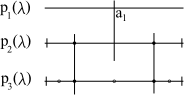
\includegraphics[scale=1.0]{capitulos/capitulo5/figuras/met_house_mat_sim1.png}
 \caption{?}
 \label{fig:met_house_mat_sim1}
\end{figure}

